\documentclass{beamer}
\usetheme{Madrid}
\usepackage{graphicx}
\setbeamertemplate{navigation symbols}{}
\setbeamertemplate{frametitle}[default][left=2cm]
\usepackage{tikz}
\usetikzlibrary{arrows.meta,positioning,fit,backgrounds,calc,shapes.geometric,decorations.pathreplacing,patterns}
\usepackage{amsmath}
\IfFileExists{usask_usask_black_reverse.png}{%
  \addtobeamertemplate{frametitle}{}{%
    \begin{tikzpicture}[remember picture,overlay]
      \node[anchor=north east,yshift=2pt,inner sep=0pt] at (current page.north east) {%
        \makebox[0pt][r]{\includegraphics[height=0.8cm]{usask_usask_black_reverse.png}}};
    \end{tikzpicture}}}{}

% colour convention
\definecolor{cW}{RGB}{50,110,200}   % weights
\definecolor{cA}{RGB}{60,170,90}    % activations
\definecolor{cG}{RGB}{240,140,30}   % gradients
\definecolor{cO}{RGB}{130,70,180}   % optimizer
\definecolor{cP}{RGB}{200,30,110}   % physics
\definecolor{cS}{RGB}{0,170,190}    % SAGE cyan
\definecolor{cY}{RGB}{225,170,0}    % SAGE gold
\tikzset{arr/.style={-{Stealth[length=2.5mm]},thick},
 box/.style={draw,rounded corners=2pt,minimum height=0.8cm,align=center,font=\small,inner sep=4pt},
 lab/.style={font=\footnotesize,align=center}}
\newcommand{\illus}[1]{\par\vfill{\tiny\color{gray}#1}}

\title[SAGE in pictures]{SAGE in Pictures}
\subtitle{Faster PINN training for battery heat-sink simulation}
\author[S. Muhsin]{Sayed Muhsin\\ Supervised by Prof. Seok-Bum Ko}
\date[2026]{November 2026}
\titlegraphic{}
\setlength{\hfuzz}{1pt}\setlength{\vfuzz}{1pt}
\begin{document}
{\hfuzz=100pt\begin{frame}\titlepage\end{frame}}

% 1 ------------------------------------------------------------
\begin{frame}{The problem: a heat sink on a big battery}
\centering
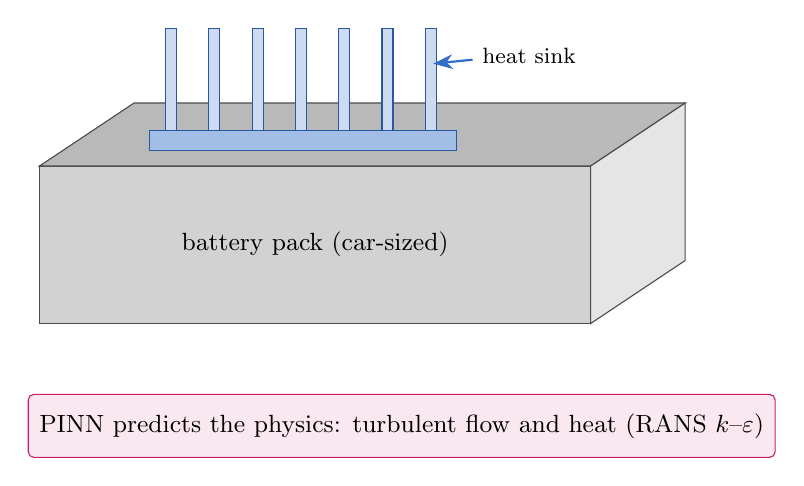
\begin{tikzpicture}[x={(1cm,0cm)},y={(0cm,1cm)}]
 % battery box (oblique)
 \def\dx{1.2}\def\dy{0.8}
 \filldraw[fill=gray!35,draw=black!70] (0,0) rectangle (7,2);
 \filldraw[fill=gray!55,draw=black!70] (0,2) -- (\dx,2+\dy) -- (7+\dx,2+\dy) -- (7,2) -- cycle;
 \filldraw[fill=gray!20,draw=black!70] (7,0) -- (7+\dx,\dy) -- (7+\dx,2+\dy) -- (7,2) -- cycle;
 \node at (3.5,1) {\small battery pack (car-sized)};
 % fins on top
 \foreach \i in {0,...,6}{
   \pgfmathsetmacro{\x}{1.6+\i*0.55}
   \filldraw[fill=cW!25,draw=cW!80!black] (\x,2.45) rectangle ++(0.14,1.3);
 }
 \filldraw[fill=cW!45,draw=cW!80!black] (1.4,2.2) rectangle (5.3,2.45);
 \node[lab,anchor=west] at (5.5,3.4) {heat sink};
 \draw[arr,cW] (5.5,3.35) -- (5.0,3.3);
 \node[box,fill=cP!10,draw=cP] (p) at (4.6,-1.3) {PINN predicts the physics: turbulent flow and heat (RANS $k$--$\varepsilon$)};
\end{tikzpicture}
\end{frame}

% 2 ------------------------------------------------------------
\begin{frame}{One PINN training step}
\centering
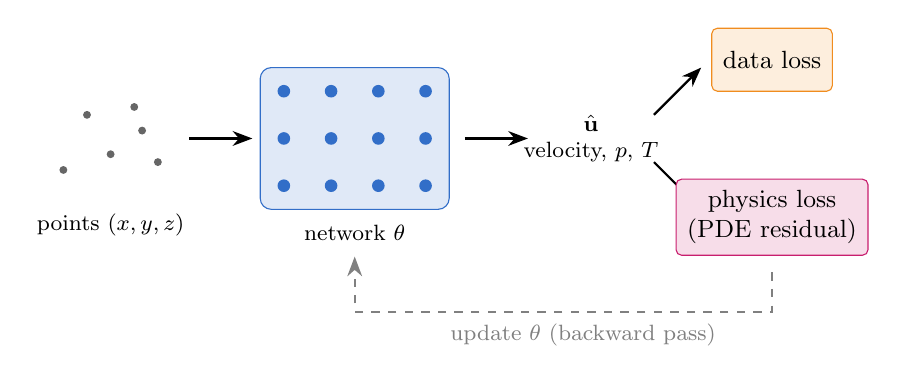
\begin{tikzpicture}
 \foreach \x/\y in {-0.3/-0.2,0/0.5,0.3/0,0.6/0.6,0.9/-0.1,0.7/0.3}{\fill[black!60] (\x,\y) circle (0.05);}
 \node[lab] at (0.3,-0.9) {points $(x,y,z)$};
 \draw[arr] (1.3,0.2)--(2.1,0.2);
 \node[draw=cW,fill=cW!15,rounded corners,minimum width=2.4cm,minimum height=1.8cm] (n) at (3.4,0.2) {};
 \foreach \l in {0,1,2,3}{\foreach \j in {0,1,2}{\fill[cW] (2.5+0.6*\l,-0.4+0.6*\j) circle (0.08);}}
 \node[lab] at (3.4,-1.0) {network $\theta$};
 \draw[arr] (4.8,0.2)--(5.6,0.2);
 \node[lab,align=center] at (6.4,0.2) {$\hat{\mathbf u}$\\ velocity, $p$, $T$};
 \draw[arr] (7.2,0.5)--(7.8,1.1); \draw[arr] (7.2,-0.1)--(7.8,-0.7);
 \node[box,fill=cG!15,draw=cG] at (8.7,1.2) {data loss};
 \node[box,fill=cP!15,draw=cP] at (8.7,-0.8) {physics loss\\ (PDE residual)};
 \draw[arr,dashed,gray] (8.7,-1.5) -- (8.7,-2.0) -- (3.4,-2.0) -- (3.4,-1.3);
 \node[lab,gray] at (6.3,-2.3) {update $\theta$ (backward pass)};
\end{tikzpicture}
\end{frame}

% 3 ------------------------------------------------------------
\begin{frame}{Where the memory goes in one step}
\centering
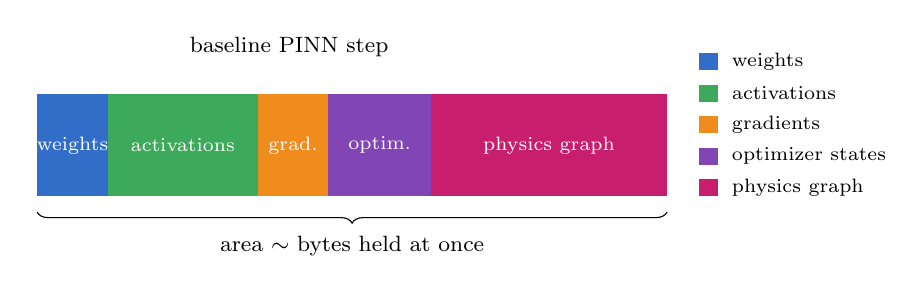
\begin{tikzpicture}
 \node[lab] at (3.2,1.9) {baseline PINN step};
 \foreach \x/\w/\c/\t in {0/0.9/cW/weights,0.9/1.9/cA/activations,2.8/0.9/cG/grad.,3.7/1.3/cO/optim.,5.0/3.0/cP/physics graph}{
   \fill[\c] (\x,0) rectangle ++(\w,1.3); \node[white,font=\scriptsize] at (\x+\w/2,0.65) {\t};}
 \draw[decorate,decoration={brace,mirror,amplitude=4pt}] (0,-0.2) -- (8,-0.2) node[midway,below=5pt,lab] {area $\sim$ bytes held at once};
 % legend
 \foreach \c/\t/\y in {cW/weights/2.2,cA/activations/1.8,cG/gradients/1.4,cO/optimizer states/1.0,cP/physics graph/0.6}{
  \fill[\c] (8.4,\y-0.6) rectangle ++(0.25,0.22); \node[lab,anchor=west,font=\scriptsize] at (8.7,\y-0.49) {\t};}
\end{tikzpicture}
\illus{Illustrative proportions, not measured.}
\end{frame}

% 4 ------------------------------------------------------------
\begin{frame}{Most of the step waits on memory}
\centering
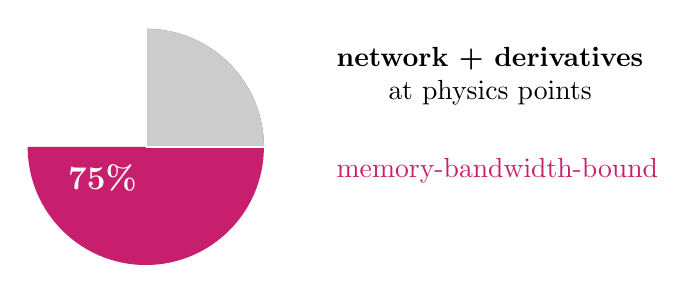
\begin{tikzpicture}
 \def\r{1.5}
 \fill[cP] (0,0) -- (0,\r) arc (90:-180:\r) -- cycle;      % 270deg = 75%
 \fill[gray!40] (0,0) -- (\r,0) arc (0:90:\r) -- cycle;
 \draw[white,thick] (0,0)--(0,\r); \draw[white,thick] (0,0)--(\r,0);
 \node[white,font=\bfseries\large] at (-0.55,-0.4) {75\%};
 \node[lab,anchor=west,font=\normalsize] at (2.3,0.9) {\textbf{network + derivatives}\\ at physics points};
 \node[lab,anchor=west,font=\normalsize,text=cP] at (2.3,-0.3) {memory-bandwidth-bound};
\end{tikzpicture}

\vspace{2mm}\small Measured, September profiling. Fix the traffic, not the maths.
\end{frame}

% 5 ------------------------------------------------------------
\begin{frame}{Weight gradient: one backward chain}
\centering
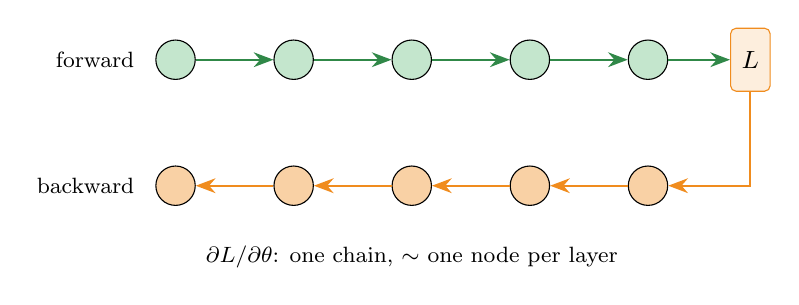
\begin{tikzpicture}[n/.style={circle,draw,minimum size=0.5cm,inner sep=0pt,font=\scriptsize}]
 \foreach \i/\c in {0/cA,1/cA,2/cA,3/cA,4/cA}{\node[n,fill=\c!30] (f\i) at (1.5*\i,1.2) {};}
 \foreach \i in {0,...,3}{\pgfmathtruncatemacro{\j}{\i+1}\draw[arr,cA!80!black] (f\i)--(f\j);}
 \node[lab,anchor=east] at (-0.4,1.2) {forward};
 \node[box,fill=cG!15,draw=cG,minimum width=0.5cm] (L) at (7.3,1.2) {$L$};
 \draw[arr,cA!80!black] (f4)--(L);
 \foreach \i in {0,...,4}{\node[n,fill=cG!40] (b\i) at (1.5*\i,-0.4) {};}
 \foreach \i in {1,...,4}{\pgfmathtruncatemacro{\j}{\i-1}\draw[arr,cG] (b\i)--(b\j);}
 \node[lab,anchor=east] at (-0.4,-0.4) {backward};
 \draw[arr,cG] (L)--(7.3,-0.4)--(b4);
 \node[lab] at (3,-1.3) {$\partial L/\partial\theta$: one chain, $\sim$ one node per layer};
\end{tikzpicture}
\end{frame}

% 6 ------------------------------------------------------------
\begin{frame}{Physics gradient: derivative of a derivative}
\centering
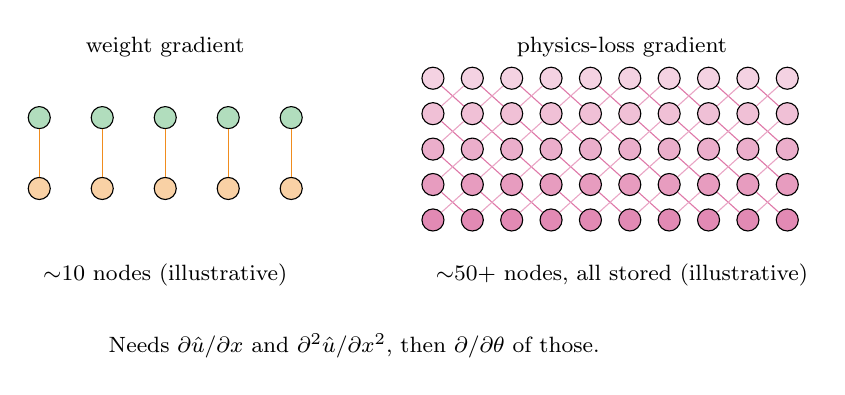
\begin{tikzpicture}[n/.style={circle,draw,minimum size=0.28cm,inner sep=0pt}]
 % left: weight graph
 \node[lab] at (1.6,3.0) {weight gradient};
 \foreach \i in {0,...,4}{\node[n,fill=cA!40] (a\i) at (0.8*\i,2.1) {};\node[n,fill=cG!40] (c\i) at (0.8*\i,1.2) {};}
 \foreach \i in {0,...,4}{\draw[cG] (a\i)--(c\i);}
 \node[lab] at (1.6,0.1) {$\sim$10 nodes (illustrative)};
 % right: physics graph
 \node[lab] at (7.4,3.0) {physics-loss gradient};
 \foreach \r in {0,...,4}{\foreach \c in {0,...,9}{
   \node[n,fill=cP!\the\numexpr 20+8*\r\relax] (p\r\c) at (5.0+0.5*\c,2.6-0.45*\r) {};}}
 \foreach \r in {0,...,3}{\pgfmathtruncatemacro{\s}{\r+1}\foreach \c in {0,...,8}{\pgfmathtruncatemacro{\d}{\c+1}
   \draw[cP!60] (p\r\c)--(p\s\d); \draw[cP!40] (p\r\d)--(p\s\c);}}
 \node[lab] at (7.4,0.1) {$\sim$50+ nodes, all stored (illustrative)};
 \node[lab] at (4,-0.8) {Needs $\partial \hat u/\partial x$ and $\partial^2 \hat u/\partial x^2$, then $\partial/\partial\theta$ of those.};
\end{tikzpicture}
\end{frame}

% 7 ------------------------------------------------------------
\begin{frame}{SAGE idea: split the gradient in two}
\centering
{\Large $\displaystyle \frac{\partial L}{\partial\theta}\;=\;\underbrace{\mathbf v}_{\partial L/\partial\hat{\mathbf u}}\;\cdot\;\underbrace{J}_{\partial\hat{\mathbf u}/\partial\theta}$}

\vspace{4mm}
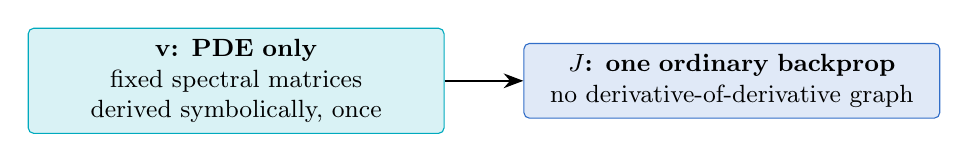
\begin{tikzpicture}
 \node[box,fill=cS!15,draw=cS,minimum width=5.2cm,text width=5cm] (v) {\textbf{$\mathbf v$: PDE only}\\ fixed spectral matrices\\ derived symbolically, once};
 \node[box,fill=cW!15,draw=cW,minimum width=5.2cm,text width=5cm,right=1.0cm of v] (j) {\textbf{$J$: one ordinary backprop}\\ no derivative-of-derivative graph};
 \draw[arr] (v)--(j);
\end{tikzpicture}

\vspace{3mm}\footnotesize Prerequisite: DT-PINN, derivatives as fixed matrices.
\end{frame}

% 8 ------------------------------------------------------------
\begin{frame}{How $\mathbf v$ is derived (once, before training)}
\centering
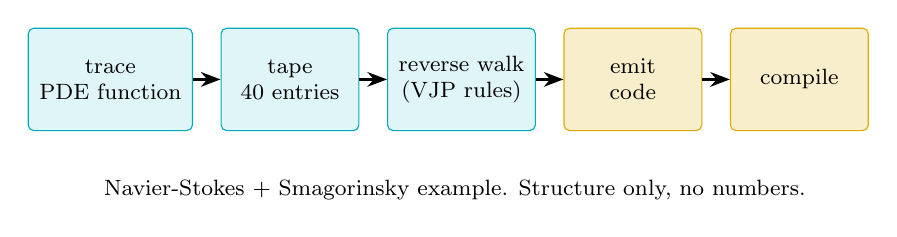
\begin{tikzpicture}[st/.style={box,fill=cS!12,draw=cS,minimum width=1.75cm,minimum height=1.3cm,font=\footnotesize}]
 \node[st] (a) {trace\\ PDE function};
 \node[st,right=0.35cm of a] (b) {tape\\ 40 entries};
 \node[st,right=0.35cm of b] (c) {reverse walk\\ (VJP rules)};
 \node[st,right=0.35cm of c,fill=cY!20,draw=cY] (d) {emit\\ code};
 \node[st,right=0.35cm of d,fill=cY!20,draw=cY] (e) {compile};
 \foreach \x/\y in {a/b,b/c,c/d,d/e}{\draw[arr] (\x)--(\y);}
 \node[lab] at ($(a)!0.5!(e)+(0,-1.4)$) {Navier-Stokes + Smagorinsky example. Structure only, no numbers.};
\end{tikzpicture}
\end{frame}

% 9 ------------------------------------------------------------
\begin{frame}{Before and after}
\centering
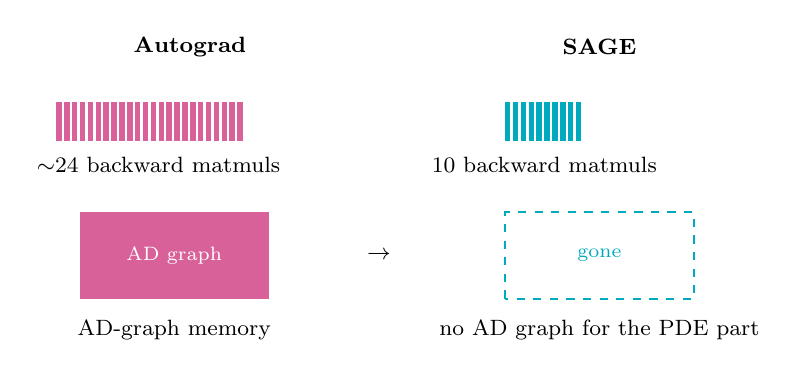
\begin{tikzpicture}
 \node[lab] at (1.4,3.2) {\textbf{Autograd}};
 \node[lab] at (6.6,3.2) {\textbf{SAGE}};
 % backward matmuls bars (24 vs 10)
 \foreach \i in {0,...,23}{\fill[cP!70] (0.1*\i-0.3,2.0) rectangle ++(0.07,0.5);}
 \foreach \i in {0,...,9}{\fill[cS] (0.1*\i+5.4,2.0) rectangle ++(0.07,0.5);}
 \node[lab] at (1.0,1.7) {$\sim$24 backward matmuls};
 \node[lab] at (5.9,1.7) {10 backward matmuls};
 % memory block
 \fill[cP!70] (0,0) rectangle (2.4,1.1); \node[white,font=\scriptsize] at (1.2,0.55) {AD graph};
 \draw[dashed,cS,thick] (5.4,0) rectangle (7.8,1.1);
 \node[cS,font=\scriptsize] at (6.6,0.55) {gone};
 \node[lab] at (3.8,0.55) {$\rightarrow$};
 \node[lab] at (1.2,-0.4) {AD-graph memory};
 \node[lab] at (6.6,-0.4) {no AD graph for the PDE part};
\end{tikzpicture}
\end{frame}

% 10 -----------------------------------------------------------
\begin{frame}{September: less memory traffic, faster step}
\centering
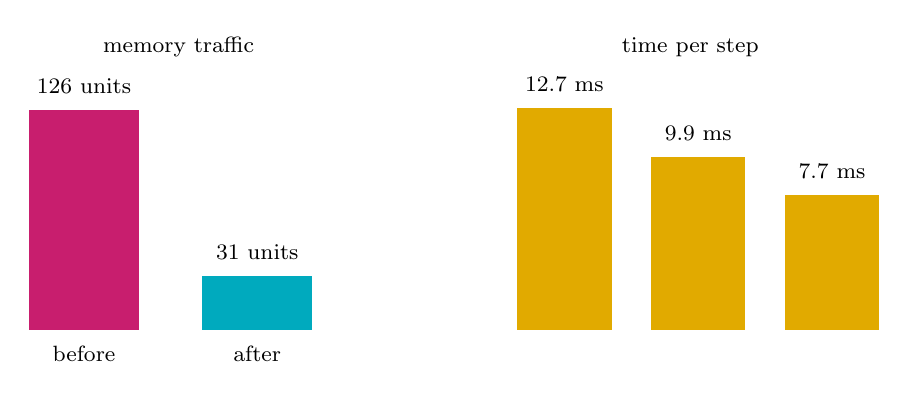
\begin{tikzpicture}
 \foreach \v/\t/\x in {126/before/0,31/after/2.2}{
   \pgfmathsetmacro{\h}{\v/45}
   \fill[\ifnum\v>100 cP\else cS\fi] (\x,0) rectangle ++(1.4,\h);
   \node[lab] at (\x+0.7,\h+0.3) {\v\ units};
   \node[lab] at (\x+0.7,-0.3) {\t};}
 \node[lab] at (1.9,3.6) {memory traffic};
 \foreach \v/\x in {12.7/6.2,9.9/7.9,7.7/9.6}{
   \pgfmathsetmacro{\h}{\v/4.5}
   \fill[cY] (\x,0) rectangle ++(1.2,\h); \node[lab] at (\x+0.6,\h+0.3) {\v\ ms};}
 \node[lab] at (8.4,3.6) {time per step};
\end{tikzpicture}

\small Measured, September deck.
\end{frame}

% 11 -----------------------------------------------------------
\begin{frame}{October: results in the UofW code}
\centering
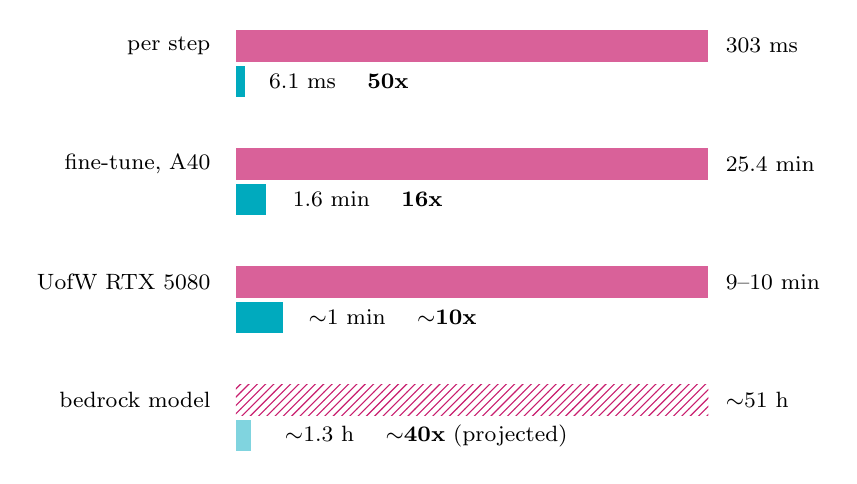
\begin{tikzpicture}
 \tikzset{bb/.style={minimum height=0.55cm,inner sep=0pt}}
 \node[lab,anchor=east] at (2.3,2.4) {per step};
 \fill[cP!70] (2.5,2.2) rectangle ++(6.0,0.4); \node[lab,anchor=west] at (8.6,2.4) {303 ms};
 \fill[cS] (2.5,1.75) rectangle ++(0.12,0.4); \node[lab,anchor=west] at (2.8,1.95) {6.1 ms \quad \textbf{50x}};
 \node[lab,anchor=east] at (2.3,0.9) {fine-tune, A40};
 \fill[cP!70] (2.5,0.7) rectangle ++(6.0,0.4); \node[lab,anchor=west] at (8.6,0.9) {25.4 min};
 \fill[cS] (2.5,0.25) rectangle ++(0.38,0.4); \node[lab,anchor=west] at (3.1,0.45) {1.6 min \quad \textbf{16x}};
 \node[lab,anchor=east] at (2.3,-0.6) {UofW RTX 5080};
 \fill[cP!70] (2.5,-0.8) rectangle ++(6.0,0.4); \node[lab,anchor=west] at (8.6,-0.6) {9--10 min};
 \fill[cS] (2.5,-1.25) rectangle ++(0.6,0.4); \node[lab,anchor=west] at (3.3,-1.05) {$\sim$1 min \quad $\sim$\textbf{10x}};
 \node[lab,anchor=east] at (2.3,-2.1) {bedrock model};
 \fill[cP!70,pattern=north east lines,pattern color=cP] (2.5,-2.3) rectangle ++(6.0,0.4); \node[lab,anchor=west] at (8.6,-2.1) {$\sim$51 h};
 \fill[cS!50] (2.5,-2.75) rectangle ++(0.19,0.4); \node[lab,anchor=west] at (3.0,-2.55) {$\sim$1.3 h \quad $\sim$\textbf{40x} (projected)};
\end{tikzpicture}

{\footnotesize Setup time (12 min bedrock, 1 min fine-tune) is not accelerated. Bedrock figures are projected.}
\end{frame}

% 12 -----------------------------------------------------------
\begin{frame}{Live demo}
\centering\vspace{6mm}

\begin{tikzpicture}
 \node[box,fill=cS!12,draw=cS,very thick,minimum width=8cm,minimum height=2.2cm,font=\Large] {One training step in 3D\\[2mm] {\normalsize toggle SAGE on and off}};
\end{tikzpicture}

\vspace{4mm}\large Open \texttt{demo/index.html}
\end{frame}

% 13 -----------------------------------------------------------
\begin{frame}{Who does what}
\centering
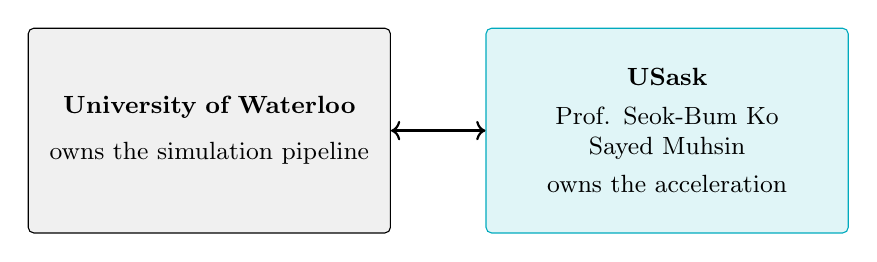
\begin{tikzpicture}
 \node[box,fill=gray!12,minimum width=4.6cm,minimum height=2.6cm,text width=4.3cm] (u) {\textbf{University of Waterloo}\\[2mm] owns the simulation pipeline};
 \node[box,fill=cS!12,draw=cS,minimum width=4.6cm,minimum height=2.6cm,text width=4.3cm,right=1.2cm of u] (s) {\textbf{USask}\\[1mm] Prof. Seok-Bum Ko\\ Sayed Muhsin\\[1mm] owns the acceleration};
 \draw[arr,<->] (u)--(s);
\end{tikzpicture}

\vspace{4mm}\small Next: support UofW's first full bedrock run; report its measured speedup.
\end{frame}

\end{document}
